\documentclass[a4paper,12pt]{report}

\usepackage{alltt, fancyvrb, url}
\usepackage{graphicx}
\usepackage{subfigure}
\usepackage{array}
\usepackage{wrapfig}
\usepackage{algorithmic}
\usepackage[utf8]{inputenc}
\usepackage{fontenc}
\usepackage{amsmath,stmaryrd,mathtools,algorithm}
\usepackage{amssymb}
\usepackage{float}
\usepackage{hyperref}

\begin{document}

    
	\title{Elaborato per il corso di Basi di dati}
	\author{
      Davide Carità - 0000873616\\
      \texttt{davide.carita@studio.unibo.it}
      \and
      Pietro Olivi - 0001020332\\
      \texttt{pietro.olivi2@studio.unibo.it}
      \and
      Lorenzo Dalmonte - 0001021552\\
      \texttt{lorenzo.dalmonte4@studio.unibo.it}
    }
	\date{}
	
    \maketitle
	\tableofcontents*
	\newpage

	\chapter{Analisi dei requisiti}

        \section{Requisiti in linguaggio naturale}
    	
        Si vuole realizzare una base di dati che supporti le funzionalità di un' applicazione di compravendita di immobili nonché il monitoraggio del welfare delle principali città europee. All'interno dell'applicazione, si potrà creare un account che permetta agli utenti di promuovere e vendere le loro proprietà attraverso la piattaforma. Allo stesso tempo, gli utenti potranno utilizzare l'applicazione per cercare e visualizzare annunci immobiliari disponibili. \\ \\ Uno dei servizi sarà quello di individuare la città europea che meglio si adatta alle proprie esigenze: si potrà vedere ad esempio quale città ha ottenuto i migliori punteggi a livello europeo in tema di qualità dell'aria, costo della vita o efficienza sanitaria. Oltre a ciò, saranno disponibili anche i dati relativi agli anni precedenti, in modo da avere uno storico che permetta di valutare lo sviluppo del welfare nella città selezionata. 
        Una volta che gli utenti hanno individuato la propria città ideale, il servizio offrirà la possibilità di visualizzare annunci immobiliari specifici suddivisi per diverse zone all'interno della città. 
        Questa suddivisione permette agli utenti di esplorare le opzioni abitative in aree specifiche che potrebbero essere più in linea con le loro preferenze e esigenze. \\ \\ Gli annunci immobiliari saranno suddivisi in tre tipi: vendita, affitto e asta, e forniranno dettagli completi sugli immobili, compresi la metratura, il numero di stanze, il prezzo e altre informazioni pertinenti. Oltre a ciò, il servizio fornirà la funzionalità di avviare una conversazione tra acquirente e venditore, offrendo loro la possibilità di scambiarsi informazioni in modo rapido. Sarà data la possibilità ai giudici d'esecuzione di creare un account privilegiato che consentirà loro di gestire delle aste immobiliari. Questo account fornirà ai giudici strumenti e funzionalità speciali per gestire l'intero processo di vendita all'asta, inclusa la creazione e la pubblicazione degli annunci, la gestione delle offerte e altre attività correlate.

    	\section{Estrazione dei concetti principali}

        {\Large \textbf{Città}} $\rightarrow$ Le città sono suddivise in diverse zone e vengono valutate in base a parametri di welfare. Gli utenti utilizzano l'applicazione per individuare la città che meglio si adatta alle loro esigenze e preferenze abitative. \\
        \\
        {\Large \textbf{Categoria}} $\rightarrow$ Le categorie di welfare sono criteri utilizzati per valutare il benessere delle città europee. Essi includono ambiente, trasporto, economia, sanità ed istruzione. Questi parametri forniscono un quadro del livello di comfort e salute delle città. Consentono agli utenti di confrontare le città in base a questi indicatori, facilitando la scelta di una città che meglio si adatta alle proprie esigenze.
            \begin{itemize}
                \item \textbf{Ambiente}
                            Valuta la qualità ambientale delle città, con indicatori come il pm 2.5 (particolato fine) e la percentuale di spazio verde urbano.
                \item \textbf{Trasporto} 
                            Valuta l'efficienza dei sistemi di trasporto urbano, considerando il tempo medio di pendolarismo e il numero di auto per persona. Fornisce informazioni sulla congestione del traffico, sull'accessibilità e sull'efficacia delle opzioni di trasporto pubblico e privato nelle città.
                \item \textbf{Economia} 
                            Valuta la vitalità economica di una città attraverso indicatori come il PIL pro capite, lo stipendio medio e il tasso di disoccupazione. Consente inoltre di avere un'indicazione sul livello di prosperità e opportunità lavorative presenti nell'area urbana considerata.
                \item \textbf{Sanità}
                            Valuta la qualità del sistema sanitario di una città, considerando l'aspettativa di vita e il numero di ospedali per abitante. Fornisce un'indicazione sulla salute generale e sull'accessibilità alle cure mediche
                \item \textbf{Istruzione} 
                            Valuta la qualità dell'istruzione in una città, considerando la percentuale di laureati, la percentuale di diplomati e il numero di università presenti oltre che dare un'indicazione sulla disponibilità e l'accessibilità all'istruzione superiore e alla formazione professionale nell'area urbana considerata.
                \end{itemize} 
        {\Large \textbf{Immobile}} $\rightarrow$ Un immobile si riferisce a una proprietà che può essere promossa, venduta, affittata o messa all'asta dagli utenti attraverso la piattaforma. Gli annunci immobiliari includono informazioni come la metratura, il numero di stanze, il prezzo e altre caratteristiche rilevanti dell'immobile. \\
        \\
        {\Large \textbf{Annuncio}} $\rightarrow$ Una presentazione di un immobile disponibile per la vendita, l'affitto o l'asta. Gli annunci forniscono dettagli completi sull'immobile, come la sua ubicazione, le specifiche, i prezzi e altre informazioni pertinenti. Gli utenti utilizzano l'applicazione per cercare, visualizzare e interagire con gli annunci immobiliari. \\
        \\
        {\Large \textbf{Account}} $\rightarrow$ Gli utilizzatori possono creare un account utente per promuovere e vendere le loro proprietà, cercare annunci immobiliari disponibili, avviare conversazioni con acquirenti o venditori e gestire altre attività correlate. Ai giudici d'esecuzione viene fornita la possibilità di creare un account privilegiato con strumenti e funzionalità speciali per gestire le aste immobiliari e le attività associate al processo di vendita all'asta. \\
        \\
        \textbf{Di seguito le principali azioni richieste:}
        
        \begin{enumerate}
        \item Creare un account utente.
        \item Pubblicare un annuncio immobiliare di vendita/affitto/asta.
        \item Visualizzare annunci immobiliari disponibili.
        \item Mostrare dettagli completi di un immobile.
        \item Avviare una conversazione con un venditore.
        \item Visualizzare punteggi di welfare di una città.
        \item Filtrare annunci immobiliari per criteri (es. prezzo, dimensioni).
        \end{enumerate}


	\chapter{Progettazione concettuale}
        La progettazione concettuale, derivata dall'analisi dei concetti principali del dominio,
        è stata incrementale in termini di complessità. Di seguito passeremo quindi in rassegna
        gli stadi dello schema cronologicamente ordinati, illustrando le motivazioni che hanno 
        portato ad effettuare i vari raffinamenti. 

        \section{Schema scheletro}
        Il primo schema è il risultato della trasposizione su E/R delle astrazioni formulate nel capitolo precedente.
        In primo piano figura l'entita \textit{città}, caratterizzata da al più N \textit{valutazioni} generiche,
        ciascuna delle quali espressa con un punteggio intero nell'intervallo [0,10]. \\
        \\
        La città è identificata da un codice univoco, in modo da evitare di incappare in uno dei ricorrenti scenari di 
        città omonime nella medesima nazione (dove lo stato ed il nome della città non sarebbero sufficienti a distinguerle). Sebbene in molti casi ciò possa essere risolto specificando la regione di appartenenza 
        delle città "doppione", rimarrebbero comunque insolute casistiche tipiche del territorio britannico, dove città omonime 
        potrebbero situarsi in contee diverse ma all'interno della stessa "Government Office \textit{Region}". A titolo di esempio, basti
        pensare che nell'intero UK compaiono 14 città chiamate Newport! \footnote{https://www.southwalesargus.co.uk/news/19433701.newports-across-world/} \\
        \\
        Un annuncio riguarda un solo immobile, mentre lo stesso immobile può comparire in più annunci diversi. Quest'ultima cardinalità,
        meno ovvia, deriva dall'esigenza di conservare lo storico di tutte le vendite/affitti di ciascuna abitazione, in modo da formulare
        in seguito un trend del prezzo in funzione del tempo (da presentare agli interessati).

        \begin{figure}[ht]
            \centering{}
            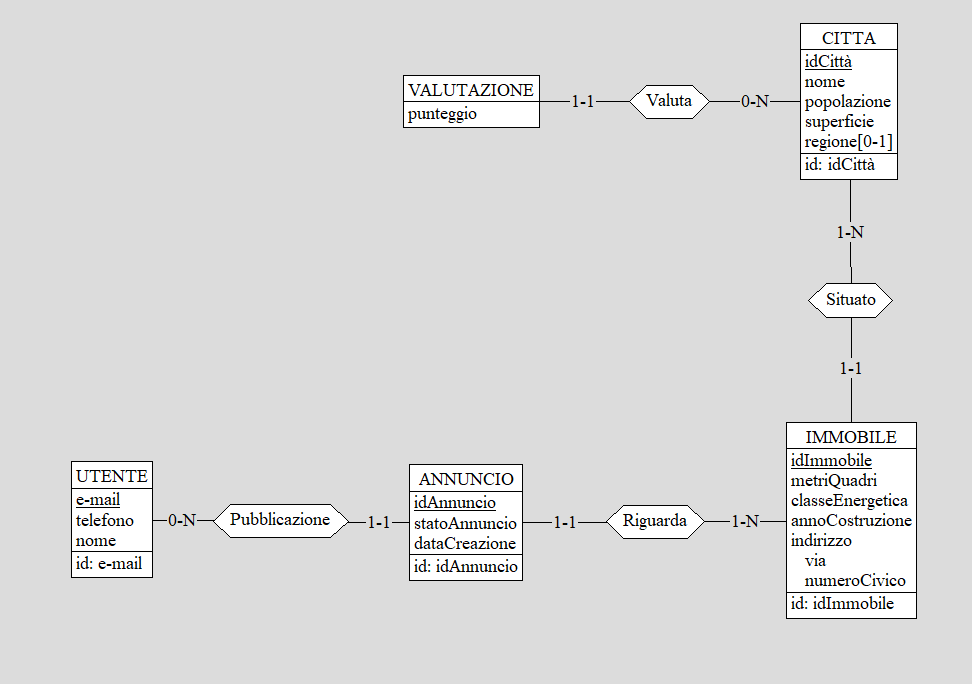
\includegraphics[width=\linewidth]{./images/first.png}
            \caption{La prima versione dello schema concettuale}
        \end{figure}

        \section{Divisione in zone e di immobili}
        
        ...

        Introducendo una gerarchia per differenziare le varie tipologie di \textit{immobili} inserite negli annunci,
        ogni immobile dovrà essere necessariamente contraddistinto da un ID proprio. Perchè? Se tutte le dimore
        fossero case indipendenti, allora potrebbero essere identificate da attributi che ne specifichino la posizione.
        Aggiungendo gli appartamenti poi, basterebbe includere nella chiave un campo che indichi il numero dell'interno.
        Con l'avvento delle stanze singole tuttavia, la soluzione precedentemente adottata risulterà inadatta, poichè 
        non risponderebbe alla necessità di un utente di affittare più stanze della stessa abitazione (ognuna con un 
        annuncio dedicato).

        \begin{figure}[ht]
            \centering{}
            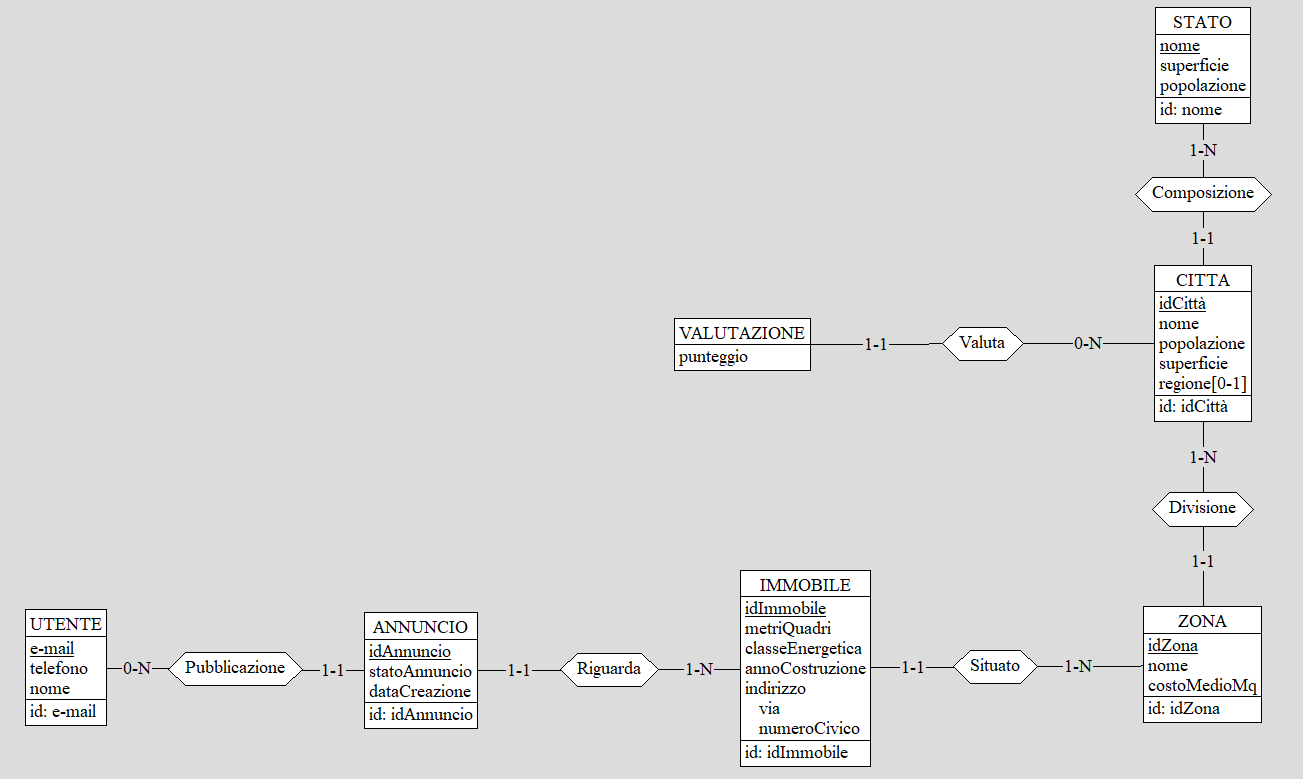
\includegraphics[width=\linewidth]{./images/second.png}
            \caption{La seconda versione dello schema concettuale}
        \end{figure}

        \section{Espansione delle valutazioni}
        Nell’amplificazione della porzione di schema relativa all’analisi delle città abbiamo scisso la precedente entità 
        “segnaposto” \textit{valutazione} in una serie di categorie, come illustrato nei requisiti. Ciascuna di queste è caratterizzata 
        da parametri dal dominio numerico (e.g. \textit{ambiente} da \textit{PM2.5media} e \textit{percentualeSpazioVerdeUrbano}), in
        base ai cui valori verrà calcolato in automatico un punteggio onnicomprensivo per la categoria, poi conservato nel campo 
        corrispondente di \textit{città\textunderscore anno} (\textit{punteggioAmbiente} nell’esempio citato). \\
        \\
        Il ruolo dell’entità \textit{città\_anno} è quello di consentire la storicizzazione dei punteggi ottenuti da ciascuna città 
        negli anni passati, in modo da poter computare lo sviluppo, o l’involuzione, a cui il luogo ha assistito. Ciascuna istanza 
        di categoria può far riferimento a più città ed in più anni diversi: Parigi e Londra potrebbero aver registrato stessi 
        \textit{PILProCapite, stipendioMedio e tassoDisoccupazione} nel 2019, così come Heidelberg potrebbe aver riconfermato gli 
        stessi valori relativi alla \textit{sanità} dell'anno precedente. Ad ogni \textit{città\_anno}, invece, è collegata una ed 
        una sola istanza di tutte le 5 categorie. \\
        \\
        
        \begin{figure}[ht]
            \centering{}
            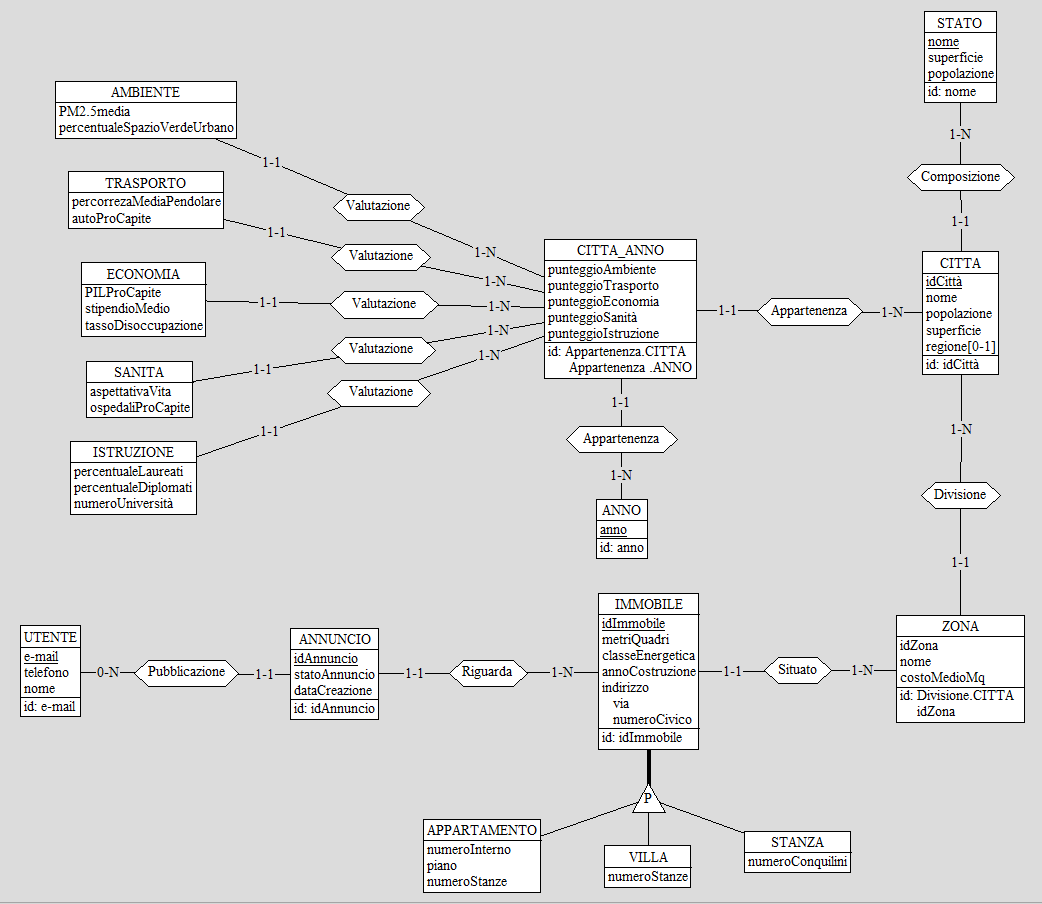
\includegraphics[width=\linewidth]{./images/third.png}
            \caption{La terza versione dello schema concettuale}
        \end{figure}
        	
    	\section{Schema finale}
        La messaggistica viene modellata attraverso le associazioni tra le entità \textit{utente $\Leftrightarrow$ messaggio} e 
        \textit{messaggio $\Leftrightarrow$ annuncio\_utente}. In prima battuta ci si potrebbe erroneamente domandare il motivo 
        del non aver optato per una relazione ad anello tra \textit{utenti}, con il testo del messaggio racchiuso in un campo 
        dell’ associazione, tuttavia tale configurazione consentirebbe di memorizzare nella base di dati al più un 
        \textit{messaggio} per ogni coppia di utenti! \\
        \\
        Sarebbe inoltre fuorviante collegare ogni messaggio direttamente 
        a mittente e destinatario poiché non si terrebbe conto del caso in cui le stesse due persone dovessero contattarsi in merito ad annunci 
        diversi, anche contemporaneamente, e non si riuscirebbe dunque a dedurre il contesto dei messaggi. Per risolvere quest’ultima problematica 
        si è deciso di interporre l'enitità \textit{messaggio} tra \textit{utente}, nonchè il potenziale acquirente, ed \textit{annuncio\_utente}, 
        ossia il gestore dell’inserzione nelle vesti del suo annuncio. I messaggi all’interno di ogni chat vengono identificati dall’istante 
        temporale in cui sono inviati (timestamp). \\
        
        \\
        Le aste sono tipologie di annunci la cui gestione (dunque pubblicazione) è riservata ad i giudici di esecuzione. In particolare, ciascuna 
        asta verrà amministrata da uno ed un solo giudice, il quale però potrà dirigerne fino ad N.
        Per riprodurre le dinamiche di ascesa del prezzo ed infine di vendita, viene istituita l’entità rialzo. \\
        \\
        Durante il periodo di attività di un’asta, scandito da una data di inizio ed una di fine, gli utenti hanno la facoltà di avanzare più rialzi 
        (Il collegare direttamente utente ad asta avrebbe ristretto il numero massimo di rialzi effettuabili da un utente, nella stessa asta, ad 1).
        I rialzi ricevuti in una determinata asta sono identificati univocamente dall’ utente che li ha effettuati e l’istante temporale in cui sono 
        stati offerti. Al termine di un asta, si può risalire al prezzo di vendita, ove avvenuta, verificando il rialzo più recente ad essa collegato.



        \begin{figure}[ht]
            \centering{}
            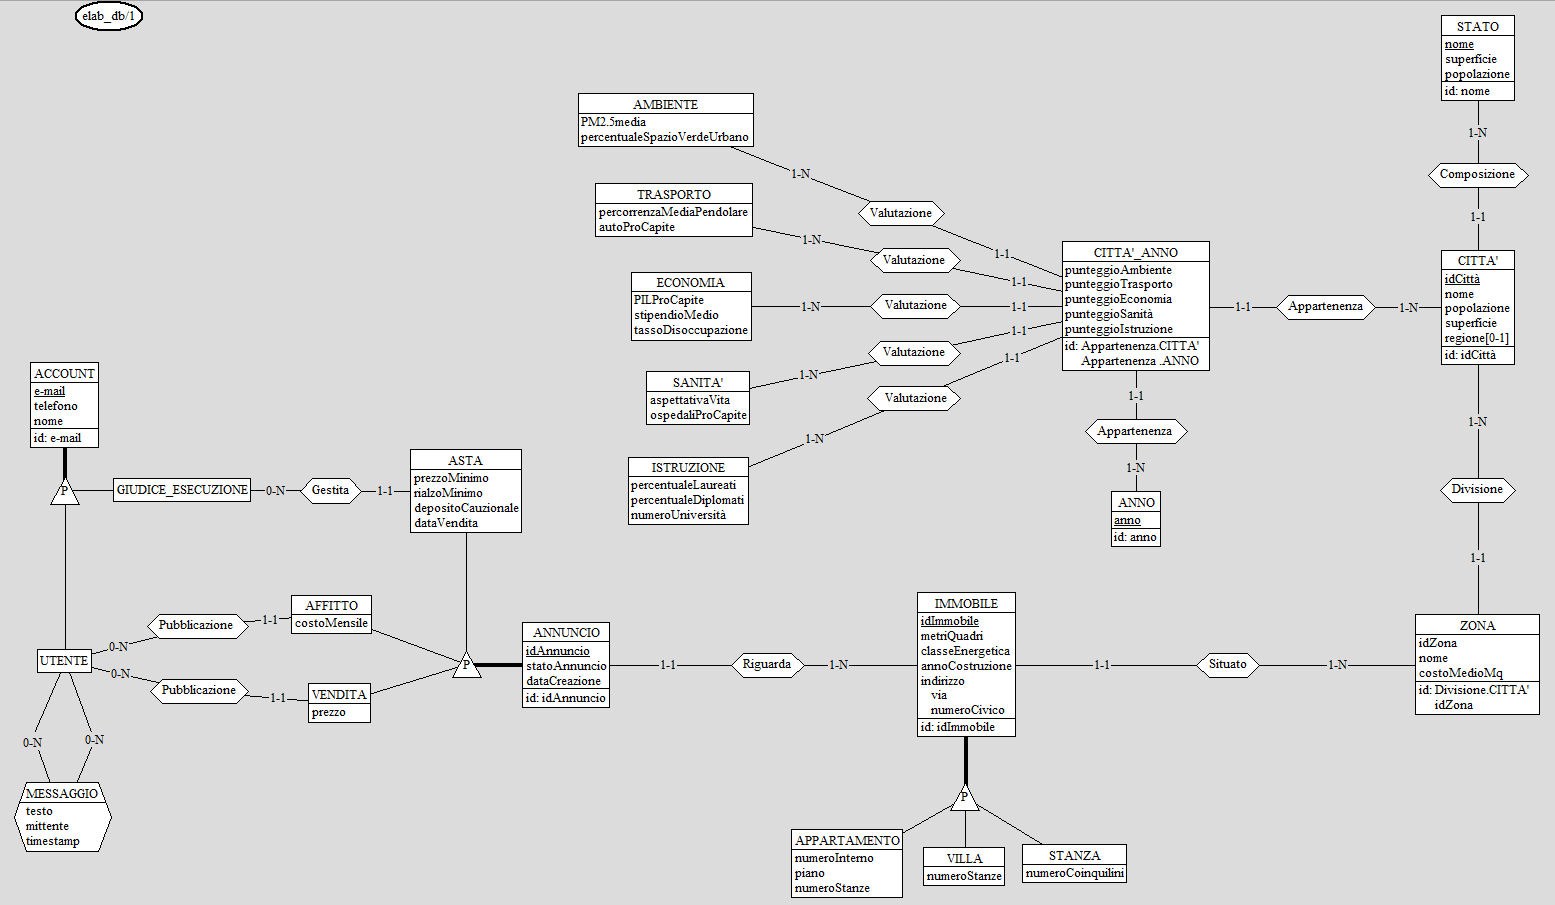
\includegraphics[width=\linewidth]{./images/fourth.png}
            \caption{L'ultima versione dello schema concettuale}
        \end{figure}

        	
	\chapter{Progettazione logica} 
    	\section{Stima del volume dei dati}
        \begin{table}[h!]
            \centering
             \begin{tabular}{||l c r||} 
             \hline
             Concetto & Costrutto & Volume \\ [0.5ex] 
             \hline\hline
             Stato & E & 50 \\
             Composizione & R & 700 \\ 
             Città & E & 700 \\
             Divisione & R & 7.000 \\
             Zona & E & 7.000 \\
             Città\_Anno & E & 14.000 \\
             Appartenenza & R & 14.000 \\
             Riferimento & R & 14.000 \\ 
             Anno & E & 20 \\
             Ambiente & E & 12.000 \\
             Valutazione\_A & R & 12.000 \\
             Trasporto & E & 12.000 \\
             Valutazione\_T & R & 12.000 \\
             Economia & E & 12.000 \\
             Valutazione\_E & R & 12.000 \\
             Sanità & E & 12.000 \\
             Valutazione\_S & R & 12.000 \\
             Istruzione & E & 12.000 \\
             Valutazione\_I & R & 12.000 \\ [1ex] 
             \hline
             \end{tabular}
        \end{table}

        \begin{table}[h!]
            \centering
             \begin{tabular}{||l c r||} 
             \hline
             Concetto & Costrutto & Volume \\ [0.5ex] 
             \hline\hline
             Situato & R & 350.000 \\
             Immobile & E & 350.000 \\
             Appartamento & E & 116.700 \\ 
             Villa & E & 116.700 \\
             Stanza & E & 116.700 \\
             Riguarda & R & 450.000 \\
             Annuncio & E & 450.000 \\
             Asta & E & 50.000 \\
             Annuncio\_Utente & E & 400.000 \\ 
             Affitto & E & 200.000 \\
             Vendita & E & 200.000 \\
             Invio/Ricezione & R & 15.000.000 \\
             Ricezione/Invio & R & 15.000.000 \\
             Messaggio & E & 15.000.000 \\
             Pubblicazione & R & 400.000 \\
             Account & E & 1.505.000 \\ 
             Utente & E & 1.500.000 \\
             Offerta & R & 750.000 \\
             Rialzo & E & 750.000 \\ 
             Accoglimento & R & 750.000 \\ 
             Gestione & R & 50.000 \\ 
             Giudice\_Esecuzione & E & 5.000 \\ [1ex] 
             \hline
             \end{tabular}
        \end{table}


    	\section{Descrizione delle operazioni principali e stima della loro frequenza}
        \begin{table}[h!]
            \centering
             \begin{tabular}{||c l r||}
             \hline
             Codice & Operazione & Frequenza \\ [0.5ex] 
             \hline\hline
             1 & Registrare un nuovo utente & 1.500 al giorno \\
             2 & Pubblicare un annuncio immobiliare (vendita, affitto o asta) & 500 al giorno \\
             3 & Visualizzare annunci immobiliari di una città in ordine cronologico & 50.000 al giorno \\ 
             4 & Suddividere gli annunci in vendita, affitto o asta all'interno di una città & 35.000 al giorno \\
             5 & Distinguere immobili per tipologia (appartamento, villa o stanza) in una data città & 35.000 al giorno \\
             6 & Ordinare gli immobili in base a particolari filtri (e.g. metratura, classe energetica) & 5.000 al giorno \\
             7 & Filtrare gli immobili per zona & 40.000 al giorno \\
             8 & Ordinare gli annunci di affitto per costo mensile & 12.000 al giorno \\
             9 & Filtrare le stanze in base ad un numero massimo di coinquilini & 7.500 al giorno \\
             10 & Mostrare aste attive in una città & 7.500 al giorno \\
             11 & Ordinare le aste per prezzo attuale crescente & 4.000 al giorno \\ 
             12 & Effettuare un rialzo all'interno di un'asta (controllando la sua validità) & 500 al giorno \\
             13 & Contattare un utente in merito ad un annuncio creato & 15.000 al giorno \\
             14 & Ricostruire una conversazione tra due utenti & 30.000 al giorno \\
             15 & Andamento del prezzo di un immobile in funzione del tempo & 5.000 al giorno \\
             16 & Comparare il prezzo di un immobile al mq con quello degli immobili nella stessa zona & 10.000 al giorno \\
             17 & Comparare il prezzo di un immobile al mq con quello degli immobili nella stessa città & 7.500 al giorno \\
             18 & Comparare il prezzo medio al mq di una zona con quello della città & 3.500 al giorno \\ 
             19 & Ordinare le zone di una città per costo medio al mq & 1.500 al giorno \\
             20 & Stilare una top 5 città per una o più categorie & 3.000 al giorno \\
             21 & Classificare città in base all'evoluzione in una o più categorie rispetto all'anno precedente & 500 al giorno \\ 
             22 & Ordinare le città in base a valori specifici di una o più categorie & 1.000 al giorno \\ 
             23 & Calcolare performance di uno stato in una o più categorie (da ogni città) & 2.000 al giorno \\ [1ex] 
             \hline
             \end{tabular}
        \end{table}
        	
    	\section{Schemi di navigazione e tabelle degli accessi}
        	
        \textbf{OP 1: Registrare un nuovo utente}
        	\begin{table}[h!]
            \centering
             \begin{tabular}{||l l l l||}
             \hline
             Concetto & Costrutto & Accessi & Tipo \\ [0.5ex] 
             \hline\hline
             Account & E & 1 & Scrittura \\ 
             \hline
              &   & Totale  3.000 al giorno &  \\ [1ex] 
             \hline
             \end{tabular}
            \end{table}

            \textbf{OP 2: Pubblicare un annuncio immobiliare (vendita o affitto)}
        	\begin{table}[h!]
            \centering
             \begin{tabular}{||l l l l||}
             \hline
             Concetto & Costrutto & Accessi & Tipo \\ [0.5ex] 
             \hline\hline
             Annuncio & E & 1 & Scrittura \\ 
             Riguarda & R & 1 & Scrittura \\ 
             Immobile & E & 1 & Scrittura \\ 
             \hline
                &   & Totale  3.000 al giorno &  \\ [1ex] 
             \hline
             \end{tabular}
            \end{table}

            Questo è invece il caso in cui l'immobile è già stato inserito da annunci passati:
            
        	\begin{table}[h!]
            \centering
             \begin{tabular}{||l l l l||}
             \hline
             Concetto & Costrutto & Accessi & Tipo \\ [0.5ex] 
             \hline\hline
             Annuncio & E & 1 & Scrittura \\ 
             \hline
                &   & Totale  1.000 al giorno &  \\ [1ex] 
             \hline
             \end{tabular}
            \end{table}

            \textbf{OP 3: Visualizzare annunci immobiliari di una città in ordine cronologico}
            per ogni città, prendiamo le sue 10 zone, che hanno in media 50 immobili l'una, visto che gli annunci (450.000~) sono più degli immobili (350.000~) uso lo stesso loro rapporto (1,3 ~) per calcolare le letture che farò negli annunci
        	\begin{table}[h!]
            \centering
             \begin{tabular}{||l l l l||}
             \hline
             Concetto & Costrutto & Accessi & Tipo \\ [0.5ex] 
             \hline\hline
             Città & E & 1 & Lettura \\ 
             Divisione & R & 10 & Lettura \\ 
             Zona & E & 10 & Lettura \\ 
             Situato & R & 50 & Lettura \\ 
             Immobile & E & 50 & Lettura \\ 
             Riguarda & R & 65 & Lettura \\ 
             Annuncio & E & 65 & Lettura \\ 
             \hline
                &   & Totale  12.550.000 al giorno &  \\ [1ex] 
             \hline
             \end{tabular}
            \end{table}

            \textbf{OP 4: Suddividere gli annunci in vendita, affitto o asta all’interno di una città}
        	\begin{table}[h!]
            \centering
             \begin{tabular}{||l l l l||}
             \hline
             Concetto & Costrutto & Accessi & Tipo \\ [0.5ex] 
             \hline\hline
             Città & E & 1 & Lettura \\ 
             Divisione & R & 10 & Lettura \\ 
             Zona & E & 10 & Lettura \\ 
             Situato & R & 50 & Lettura \\ 
             Immobile & E & 50 & Lettura \\ 
             Riguarda & R & 65 & Lettura \\ 
             Annuncio & E & 65 & Lettura \\ 
             \hline
                &   & Totale  8.785.000 al giorno &  \\ [1ex] 
             \hline
             \end{tabular}
            \end{table}

            \textbf{OP 5: Distinguere immobili per tipologia (appartamento, villa o stanza) in una data città}
        	\begin{table}[h!]
            \centering
             \begin{tabular}{||l l l l||}
             \hline
             Concetto & Costrutto & Accessi & Tipo \\ [0.5ex] 
             \hline\hline
             Città & E & 1 & Lettura \\ 
             Divisione & R & 10 & Lettura \\ 
             Zona & E & 10 & Lettura \\ 
             Situato & R & 50 & Lettura \\ 
             Immobile & E & 50 & Lettura \\
             \hline
                &   & Totale  4.235.000 al giorno &  \\ [1ex] 
             \hline
             \end{tabular}
            \end{table}

            \textbf{OP 6: Ordinare gli immobili in base a particolari filtri (e.g. metratura, classe energetica)}
        	\begin{table}[h!]
            \centering
             \begin{tabular}{||l l l l||}
             \hline
             Concetto & Costrutto & Accessi & Tipo \\ [0.5ex] 
             \hline\hline
             Città & E & 1 & Lettura \\ 
             Divisione & R & 10 & Lettura \\ 
             Zona & E & 10 & Lettura \\ 
             Situato & R & 50 & Lettura \\ 
             Immobile & E & 50 & Lettura \\
             \hline
                &   & Totale  605.000 al giorno &  \\ [1ex] 
             \hline
             \end{tabular}
            \end{table}

            \textbf{OP 7: Filtrare gli immobili per zona}
        	\begin{table}[h!]
            \centering
             \begin{tabular}{||l l l l||}
             \hline
             Concetto & Costrutto & Accessi & Tipo \\ [0.5ex] 
             \hline\hline
             Città & E & 1 & Lettura \\ 
             Divisione & R & 10 & Lettura \\ 
             Zona & E & 10 & Lettura \\ 
             Situato & R & 50 & Lettura \\ 
             Immobile & E & 50 & Lettura \\
             \hline
                &   & Totale  4.840.000 al giorno &  \\ [1ex] 
             \hline
             \end{tabular}
            \end{table}

            \textbf{OP 8: Ordinare gli annunci di affitto per costo mensile}
        	\begin{table}[h!]
            \centering
             \begin{tabular}{||l l l l||}
             \hline
             Concetto & Costrutto & Accessi & Tipo \\ [0.5ex] 
             \hline\hline
             Città & E & 1 & Lettura \\ 
             Divisione & R & 10 & Lettura \\ 
             Zona & E & 10 & Lettura \\ 
             Situato & R & 50 & Lettura \\ 
             Immobile & E & 50 & Lettura \\ 
             Riguarda & R & 65 & Lettura \\ 
             Annuncio & E & 65 & Lettura \\ 
             \hline
                &   & Totale  3.012.000 al giorno &  \\ [1ex] 
             \hline
             \end{tabular}
            \end{table}

            \textbf{OP 9: Filtrare le stanze in base ad un numero massimo di coinquilini}
        	\begin{table}[h!]
            \centering
             \begin{tabular}{||l l l l||}
             \hline
             Concetto & Costrutto & Accessi & Tipo \\ [0.5ex] 
             \hline\hline
             Città & E & 1 & Lettura \\ 
             Divisione & R & 10 & Lettura \\ 
             Zona & E & 10 & Lettura \\ 
             Situato & R & 50 & Lettura \\ 
             Immobile & E & 50 & Lettura \\ 
             \hline
                &   & Totale  907.500 al giorno &  \\ [1ex] 
             \hline
             \end{tabular}
            \end{table}

            \textbf{OP 10: Mostrare aste attive in una città}
        	\begin{table}[h!]
            \centering
             \begin{tabular}{||l l l l||}
             \hline
             Concetto & Costrutto & Accessi & Tipo \\ [0.5ex] 
             \hline\hline
             Città & E & 1 & Lettura \\ 
             Divisione & R & 10 & Lettura \\ 
             Zona & E & 10 & Lettura \\ 
             Situato & R & 50 & Lettura \\ 
             Immobile & E & 50 & Lettura \\ 
             Riguarda & R & 65 & Lettura \\ 
             Annuncio & E & 65 & Lettura \\ 
             \hline
                &   & Totale  907.500 al giorno &  \\ [1ex] 
             \hline
             \end{tabular}
            \end{table}

            \textbf{OP 11: Ordinare le aste per prezzo attuale crescente}
        	\begin{table}[h!]
            \centering
             \begin{tabular}{||l l l l||}
             \hline
             Concetto & Costrutto & Accessi & Tipo \\ [0.5ex] 
             \hline\hline
             Città & E & 1 & Lettura \\ 
             Divisione & R & 10 & Lettura \\ 
             Zona & E & 10 & Lettura \\ 
             Situato & R & 50 & Lettura \\ 
             Immobile & E & 50 & Lettura \\ 
             Riguarda & R & 65 & Lettura \\ 
             Annuncio & E & 65 & Lettura \\ 
             \hline
                &   & Totale  1.004.000 al giorno &  \\ [1ex] 
             \hline
             \end{tabular}
            \end{table}

            \textbf{OP 12: Effettuare un rialzo all’interno di un’asta (controllando la sua validità)}
        	\begin{table}[h!]
            \centering
             \begin{tabular}{||l l l l||}
             \hline
             Concetto & Costrutto & Accessi & Tipo \\ [0.5ex] 
             \hline\hline
             Account & E & 1 & Lettura \\ 
             Offerta & R & 1 & Lettura \\ 
             Rialzo & E & 1 & Lettura \\ 
             Riceve & R & 1 & Lettura \\ 
             Annuncio & E & 1 & Lettura \\ 
             Offerta & R & 1 & Scrittura \\ 
             Rialzo & E & 1 & Scrittura \\ 
             Riceve & R & 1 & Scrittura \\ 
             \hline
                &   & Totale  5.500 al giorno &  \\ [1ex] 
             \hline
             \end{tabular}
            \end{table}

            \textbf{OP 13: Contattare un utente in merito ad un annuncio creato}
        	\begin{table}[h!]
            \centering
             \begin{tabular}{||l l l l||}
             \hline
             Concetto & Costrutto & Accessi & Tipo \\ [0.5ex] 
             \hline\hline
             Account & E & 1 & Lettura \\ 
             Annuncio & E & 1 & Lettura \\ 
             Invio/Ricezione & R & 1 & Scrittura \\ 
             Messaggio & E & 1 & Scrittura \\ 
             Invio/Ricezione & R & 1 & Scrittura \\ 
             \hline
                &   & Totale  120.000 al giorno &  \\ [1ex] 
             \hline
             \end{tabular}
            \end{table}

            \textbf{OP 14: Ricostruire una conversazione tra due utenti}
        	\begin{table}[h!]
            \centering
             \begin{tabular}{||l l l l||}
             \hline
             Concetto & Costrutto & Accessi & Tipo \\ [0.5ex] 
             \hline\hline
             Account & E & 1 & Lettura \\ 
             Annuncio & E & 1 & Lettura \\ 
             Invio/Ricezione & R & 10 & Lettura \\ 
             Messaggio & E & 10 & Lettura \\ 
             Invio/Ricezione & R & 10 & Lettura \\ 
             \hline
                &   & Totale  960.000 al giorno &  \\ [1ex] 
             \hline
             \end{tabular}
            \end{table}

             \textbf{OP 15: Andamento del prezzo di un immobile in funzione del tempo}
        	\begin{table}[h!]
            \centering
             \begin{tabular}{||l l l l||}
             \hline
             Concetto & Costrutto & Accessi & Tipo \\ [0.5ex] 
             \hline\hline
             Immobile & E & 1 & Lettura \\ 
             Riguarda & R & 1.3 & Lettura \\ 
             Annuncio & E & 1.3 & Lettura \\ 
             \hline
                &   & Totale  18.000 al giorno &  \\ [1ex] 
             \hline
             \end{tabular}
            \end{table}

            \textbf{OP 16: Comparare il prezzo di un immobile al mq con quello degli immobili nella stessa zona}
        	\begin{table}[h!]
            \centering
             \begin{tabular}{||l l l l||}
             \hline
             Concetto & Costrutto & Accessi & Tipo \\ [0.5ex] 
             \hline\hline
             Immobile & E & 1 & Lettura \\ 
             Situato & R & 1 & Lettura \\ 
             Zona & E & 1 & Lettura \\ 
             \hline
                &   & Totale  30.000 al giorno &  \\ [1ex] 
             \hline
             \end{tabular}
            \end{table}

            \textbf{OP 17: Comparare il prezzo di un immobile al mq con quello degli immobili nella stessa città}
        	\begin{table}[h!]
            \centering
             \begin{tabular}{||l l l l||}
             \hline
             Concetto & Costrutto & Accessi & Tipo \\ [0.5ex] 
             \hline\hline
             Immobile & E & 1 & Lettura \\ 
             Situato & R & 1 & Lettura \\ 
             Zona & E & 10 & Lettura \\ 
             Divisione & R & 10 & Lettura \\ 
             Città & E & 1 & Lettura \\ 
             \hline
                &   & Totale  172.500 al giorno &  \\ [1ex] 
             \hline
             \end{tabular}
            \end{table}

            \textbf{OP 18: Comparare il prezzo medio al mq di una zona con quello della città}
        	\begin{table}[h!]
            \centering
             \begin{tabular}{||l l l l||}
             \hline
             Concetto & Costrutto & Accessi & Tipo \\ [0.5ex] 
             \hline\hline
             Zona & E & 10 & Lettura \\ 
             Divisione & R & 10 & Lettura \\ 
             Città & E & 1 & Lettura \\ 
             \hline
                &   & Totale  73.500 al giorno &  \\ [1ex] 
             \hline
             \end{tabular}
            \end{table}

            \textbf{OP 19: Ordinare le zone di una città per costo medio al mq}
        	\begin{table}[h!]
            \centering
             \begin{tabular}{||l l l l||}
             \hline
             Concetto & Costrutto & Accessi & Tipo \\ [0.5ex] 
             \hline\hline
             Zona & E & 10 & Lettura \\ 
             Divisione & R & 10 & Lettura \\ 
             Città & E & 1 & Lettura \\ 
             \hline
                &   & Totale  31.500 al giorno &  \\ [1ex] 
             \hline
             \end{tabular}
            \end{table}

            \textbf{OP 20: Stilare una top 5 città per una o più categorie}
        	\begin{table}[h!]
            \centering
             \begin{tabular}{||l l l l||}
             \hline
             Concetto & Costrutto & Accessi & Tipo \\ [0.5ex] 
             \hline\hline
             Anno & E & 1 & Lettura \\ 
             Città\_Anno & E & 700 & Lettura \\ 
             Appartenenza & R & 5 & Lettura \\ 
             Città & E & 5 & Lettura \\ 
             \hline
                &   & Totale  2.133.000 al giorno &  \\ [1ex] 
             \hline
             \end{tabular}
            \end{table}

            \textbf{OP 21: Classificare città in base all’evoluzione in una o più categorie rispetto all’anno precedente}
        	\begin{table}[h!]
            \centering
             \begin{tabular}{||l l l l||}
             \hline
             Concetto & Costrutto & Accessi & Tipo \\ [0.5ex] 
             \hline\hline
             Anno & E & 2 & Lettura \\ 
             Città\_Anno & E & 1.400 & Lettura \\ 
             Appartenenza & R & 1.400 & Lettura \\ 
             Città & E & 1.400 & Lettura \\ 
             \hline
                &   & Totale  2.101.000 al giorno &  \\ [1ex] 
             \hline
             \end{tabular}
            \end{table}

            \textbf{OP 22: Ordinare le città in base a valori specifici di una o più categorie}
        	\begin{table}[h!]
            \centering
             \begin{tabular}{||l l l l||}
             \hline
             Concetto & Costrutto & Accessi & Tipo \\ [0.5ex] 
             \hline\hline
             Anno & E & 1 & Lettura \\ 
             Città\_Anno & E & 700 & Lettura \\ 
             Valutazione\_A & R & 700 & Lettura \\ 
             Ambiente & E & 700 & Lettura \\
             Valutazione\_T & R & 700 & Lettura \\ 
             Trasporto & E & 700 & Lettura \\
             Valutazione\_E & R & 700 & Lettura \\ 
             Economia & E & 700 & Lettura \\
             Valutazione\_S & R & 700 & Lettura \\ 
             Sanità & E & 700 & Lettura \\
             Valutazione\_I & R & 700 & Lettura \\ 
             Istruzione & E & 700 & Lettura \\
             \hline
                &   & Totale  7.701.000 al giorno &  \\ [1ex] 
             \hline
             \end{tabular}
            \end{table}

            \textbf{OP 23: Calcolare performance di uno stato in una o più categorie (da ogni città)}
        	\begin{table}[h!]
            \centering
             \begin{tabular}{||l l l l||}
             \hline
             Concetto & Costrutto & Accessi & Tipo \\ [0.5ex] 
             \hline\hline
             Stato & E & 1 & Lettura \\ 
             Composizione & R & 14 & Lettura \\ 
             Città & E & 14 & Lettura \\ 
             Appartenenza & R & 28 & Lettura \\ 
             Città\_Anno & E & 28 & Lettura \\ 
             \hline
                &   & Totale  170.000 al giorno &  \\ [1ex] 
             \hline
             \end{tabular}
            \end{table}
        	
    	\section{Analisi delle ridondanze}
        	asdasd
        	
    	\section{Traduzione di entità e associazioni in relazioni}
        	asdasd
        	
    	\section{Schema relazionale finale}
        	asdasd
        	
    	\section{Descrizione dell'architettura dell'applicazione realizzata}
        	asdasd
        	

    \addcontentsline{toc}{chapter}{Progettazione dell'applicazione}
	\chapter*{Progettazione dell'applicazione}
	
    	\addcontentsline{toc}{section}{Traduzione delle operazioni in query SQL} 
    	\section*{Traduzione delle operazioni in query SQL}
    	    asdasd
 
\end{document}